\documentclass[../primer.tex]{subfiles}

\begin{document}

\chapter{Wrangle}
%% --------------------------------------------------
After clearly formulating our question(s), finding and exploring the available
data, obtaining and assessing a relevant model, we may proceed to
\textbf{wrangling} the uncertainty.

If we are pursuing a predictive simulation, we might carry out \textbf{forward
  propagation} -- compute the uncertainty in $Y$ based on the input uncertainty
in $\mX$. We might use the same techniques to support model validation.

If we are attempting to determine some un-measurable physical quantity with the
aid of a model and physical data, we might carry out \textbf{inverse
  propagation}, also called inference.

The forward and reverse problems are rather different in character, but both
are affected by the \textbf{curse of dimensionality}.

\section{Dimensionality}
%% --------------------------------------------------
The \textbf{curse of
  dimensionality}\footnote{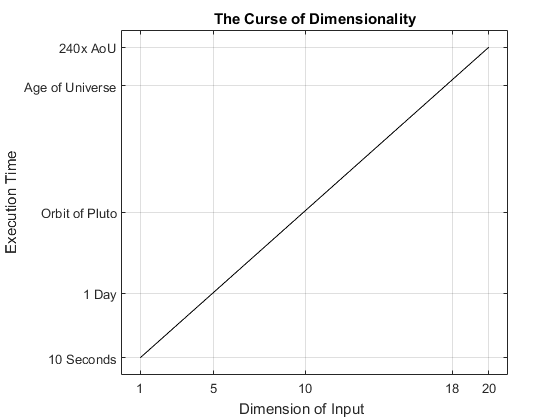
\includegraphics[width=0.50\textwidth]{./images/curse_of_dimensionality}\\ Recall
  that na\"ive execution time scales \emph{exponentially} with the number of
  dimensions.} manifests in many ways,

\section{Forward}
%% --------------------------------------------------

\section{Inverse}
%% --------------------------------------------------

\end{document}
